\section{Transição Demográfica} \label{sec:transicao}

O Brasil atravessa uma transição demográfica acelerada: a população de 0–14 anos está em queda contínua, enquanto a de 60 anos ou mais cresce rapidamente, com o ponto de cruzamento previsto por volta de 2029. Esse envelhecimento traz implicações profundas para diferentes dimensões de política pública, inclusive a Educação Profissional e Tecnológica (EPT).


\subsection{Implicações para EPT}

Em primeiro lugar, impõe a necessidade de políticas de requalificação e educação ao longo da vida, já que a força de trabalho será proporcionalmente menor e precisará ser mais produtiva. O crescimento da produtividade no Brasil tem mostrado sinais de estagnação, e esse contexto coloca ainda mais pressão sobre a qualificação dos trabalhadores, tornando a EPT um instrumento essencial para sustentar o desenvolvimento econômico.

\begin{figure}[htbp!]
	\centering
	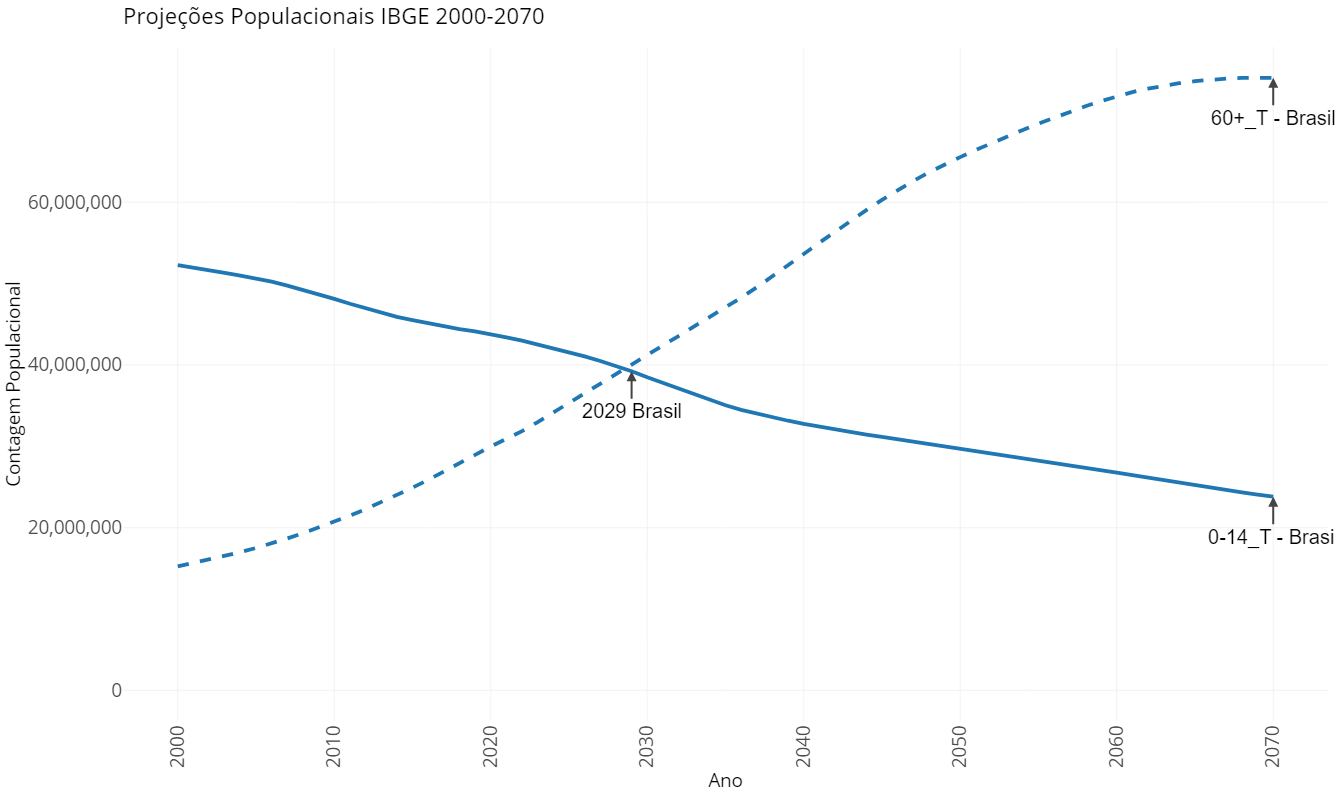
\includegraphics[width=0.75\textwidth]{images/2a_PopuBra.png}
	\caption{Transição demográfica no Brasil: evolução das populações de 0-14 e 60+ anos (2000-2070)} 
	\label{fig:2a_PopuBra}
\end{figure}

Em segundo lugar, o envelhecimento populacional impacta diretamente a demanda por serviços sociais, sobretudo saúde, cuidados de longa duração e apoio ao idoso. Isso cria tanto oportunidades quanto necessidades de formação em ocupações ligadas a serviços de cuidado, assistência e saúde. Ao mesmo tempo, avanços médicos e hábitos de vida mais saudáveis permitem que pessoas idosas permaneçam ativas por mais tempo, o que reforça a importância da requalificação e do reingresso no mercado de trabalho para essa faixa etária.

Por fim, é importante notar que essa transição não ocorre de forma homogênea no território brasileiro: estados com população jovem por mais tempo enfrentam o desafio imediato de expandir a oferta de EPT para absorver grandes coortes de jovens, enquanto estados já envelhecidos precisam ajustar suas estratégias para equilibrar a formação inicial com programas de requalificação e atualização contínua.

\subsection{Implicações para EPT}





\begin{itemize}
\item{pellentesque habitant morbi tristique}
\item{senectus et netus et malesuada fames ac turpis egestas}
\item{ut sit amet ultricies nisl}
\item{etiam laoreet condimentum lacus et elementum}
\end{itemize}

Sed vehicula quis ligula non fermentum. Pellentesque semper ligula gravida "$C_i$",
bibendum dui ut, semper nibh. Quisque a risus porta, fermentum velit vitae,
pellentesque felis.


\begin{figure}[hb]
	\centering
\includegraphics[scale=1]{images/orange2.jpg}
	\caption{Maecenas varius orci vitae eros euismod placerat} \label{fig:integer}
\end{figure}



\newpage
\subsection{Phasellus et quam}

Suspendisse potenti. Aliquam id metus in purus imperdiet aliquam eu ut dolor :

\begin{highlight}
\begin{align}
\alpha_{i+1} &= \frac{A_{i+1}}{S_{i+1}} \\
             &= \frac{A_i + \Delta A_i}{S_i + \Delta S_i} \\
             &= \frac{A_i + \Delta A_i}{S_i + \frac{\Delta A_i}{\alpha_i}} \\
             &= \alpha_i * \frac{A_i + \Delta A_i}{\alpha_i * S_i + \Delta A_i} \\
             &= \alpha_i
\end{align}
\end{highlight}

Vestibulum luctus consectetur vestibulum. Duis ullamcorper ligula nec mauris
viverra rhoncus. Aliquam auctor est accumsan odio vehicula ornare.

\begin{remark}
Duis et metus auctor, fringilla nulla non, dapibus felis \ref{sec:proin}.
\end{remark}

Morbi ipsum dui, rutrum et cursus a, porta eu ligula. Nulla lobortis leo eget
odio bibendum rhoncus. Maecenas posuere nulla nec felis viverra blandit.

\subsection{Felis nunc}

Sit amet elementum tortor malesuada quis. Quisque pellentesque nisl quis augue
interdum vehicula. Nunc nec dictum sem. Nunc venenatis elementum hendrerit \href{https://example.com/}{example.com}.

\begin{remark}
Pellentesque ut justo arcu. Fusce cursus luctus tortor eu venenatis.
\end{remark}

Maecenas viverra dui vitae eros tristique, porta elementum mi aliquam. Cras
sodales erat et molestie auctor. Phasellus mauris eros, bibendum sit amet
rhoncus id, bibendum ut velit.
